%
%===============>>  ГРУППА 11-1 МОДУЛЬ 8  <<=============
%
\setmodule{8}

%BEGIN_FOLD % ====>>_____ Занятие 1 _____<<====
\begin{class}[number=1]
	\begin{listofex} %Взяты 222 a 2 4 5 6 c193 25 26 a
		%\item Решите уравнения: %c51 1 2 4 5 a
		%\begin{tasks}(2)
		%	\task \( \dfrac{ x^2-9 }{ \sqrt[]{-5x} }=0 \)
		%	\task \( (x^2-16)\sqrt[]{3-x}=0 \)
		%	\task \( \dfrac{ x^2-10x+9 }{ \sqrt[]{x}-3 }=0 \)
		%	\task \( \sqrt[]{2x^2+7}=x-4 \)
		%\end{tasks}
		%\item Решите неравенства: %c193 23 24 27 28 a
		%\begin{tasks}(2)
		%	\task \( \sqrt[4]{x^2-24x} \le 3 \)
		%	\task \( \sqrt[28]{8x-x^2-15} < 1 \)
		%	\task \( \sqrt[]{x^2-2x-15} < 3 \)
		%	\task \( \sqrt[]{3x^2-14x+51} \ge 6 \)
		%\end{tasks}
		%\item Решите неравенства:
		%\begin{tasks}(1)
		%	\task \( \sqrt[]{x^4-2x+6} \ge x \)
		%	\task \( \sqrt[]{5x^4-28x^2+16} \ge x^2+4 \)
		%	\task \( \sqrt[]{x^2-17x-29} \ge 3|x+2| \)
		%\end{tasks}
		\item Вычислить: %114m3
		\begin{tasks}(2)
			\task \( \dfrac{-13\sin126\degree}{\sin54\degree} \)
			\task \( \cos^2(-46\degree)+\sin^2(-46\degree) \)
			\task \( \sin^223\degree+9+\cos^223 \)
			\task \( \dfrac{2\sin^221\degree+2\cos^221\degree}{4} \)
		\end{tasks}
		%\item Вычислить: %114m3
		%\begin{tasks}(1)
		%	%\task \( \left( \dfrac{4\tg120\degree\cdot\cos210\degree-\sin270\degree}{2\cos240\degree-3\sqrt{3}\sin210\degree} \right)\cdot\dfrac{5}{3\sqrt{3}+2}-\dfrac{1}{23} \)\answer{ \( 3 \) }
		%	\task \( \dfrac{\sqrt{8}\sin\left( -\dfrac{\pi}{4} \right)+\sqrt{27}\cos\left( \dfrac{\pi}{3} \right)-4\sin\left( -\dfrac{\pi}{6} \right)}{6\sqrt{3}} \) \answer{ \( 0,25 \) }
		%	\task \( 4\cos\left( \dfrac{2\pi}{3} \right)-\left( \sqrt{3}+1 \right)\left( \ctg\left( \dfrac{7\pi}{6} \right)-1 \right) \) \answer{ \( -4 \) }
		%	\task \( \left( 4 - \sin\left( -\dfrac{10\pi}{3} \right) \right)^2+4\tg\left( \dfrac{\pi}{3} \right) \) \answer{ \( 16,75 \) }
		%\end{tasks}
		\item Найдите значение выражения: \( \sin\left( \dfrac{\pi}{3}+\alpha \right) \), если \( \cos\alpha=-\dfrac{8}{17} \) и \\ \( \pi<\alpha<\dfrac{3\pi}{2} \).
		%\item Найдите значение выражения: \( \dfrac{2\cos^2x-7\sin^2x}{3\cos^2x+4\sin x\cdot\cos x} \), если \( \ctg x = -2 \).
		
		%\item %1 параболы
		%\begin{minipage}[t]{\bodywidth}
		%	На рисунке изображены графики функций \(f(x) = 4x^2-25x+41 \) и \( g(x)=ax^2+bx+c \), которые пересекаются в точках \(A\) и \(B\). Найдите абсциссу точки \(B\).
		%\end{minipage}
		%\hspace{0.02\linewidth}
		%\begin{minipage}[t]{\picwidth}
		%	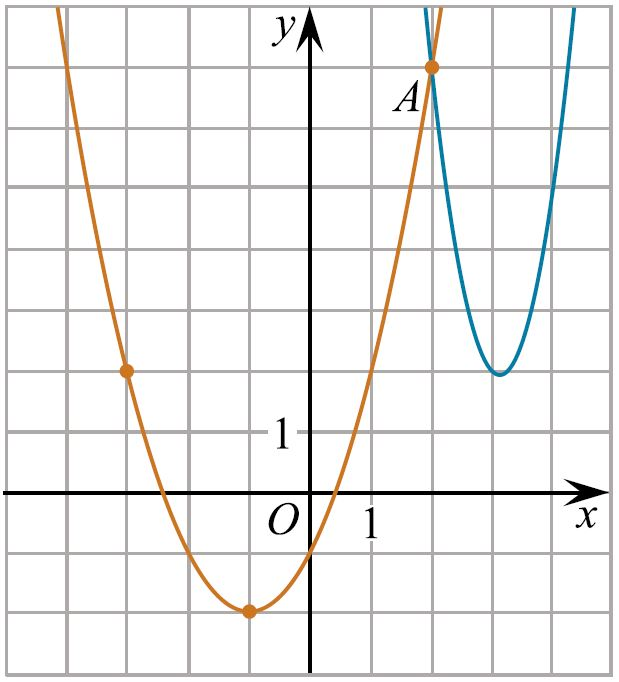
\includegraphics[align=t, width=\linewidth]{../pics/G112M3C1-10}
		%\end{minipage}
		%\item %1 LOGARIFM
		%\begin{minipage}[t]{\bodywidth}
		%	На рисунке изображен график функции \(f(x) = b+\log_ax \). Найдите \(f(32)\).
		%\end{minipage}
		%\hspace{0.02\linewidth}
		%\begin{minipage}[t]{\picwidth}
		%	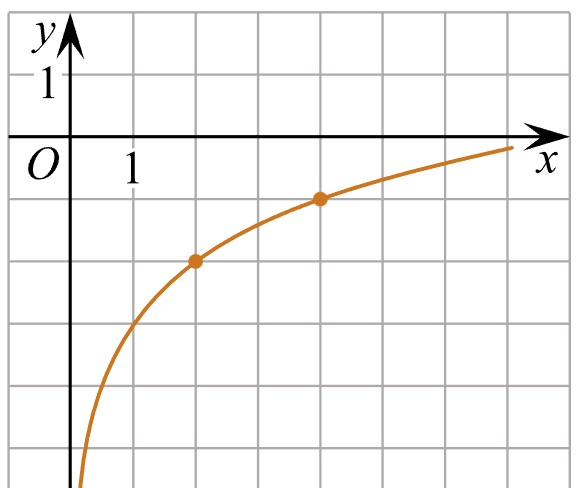
\includegraphics[align=t, width=\linewidth]{../pics/G111M8L1-1}
		%\end{minipage}
		%\item %1 s golovi
		%\begin{minipage}[t]{\bodywidth}
		%	На рисунке изображен график функции \(f(x) = \dfrac{ x^2 }{ a }+bx+c \), где числа \(a, b, c\) --- целые. Найдите значение \(f(3,5)\).
		%\end{minipage}
		%\hspace{0.02\linewidth}
		%\begin{minipage}[t]{\picwidth}
		%	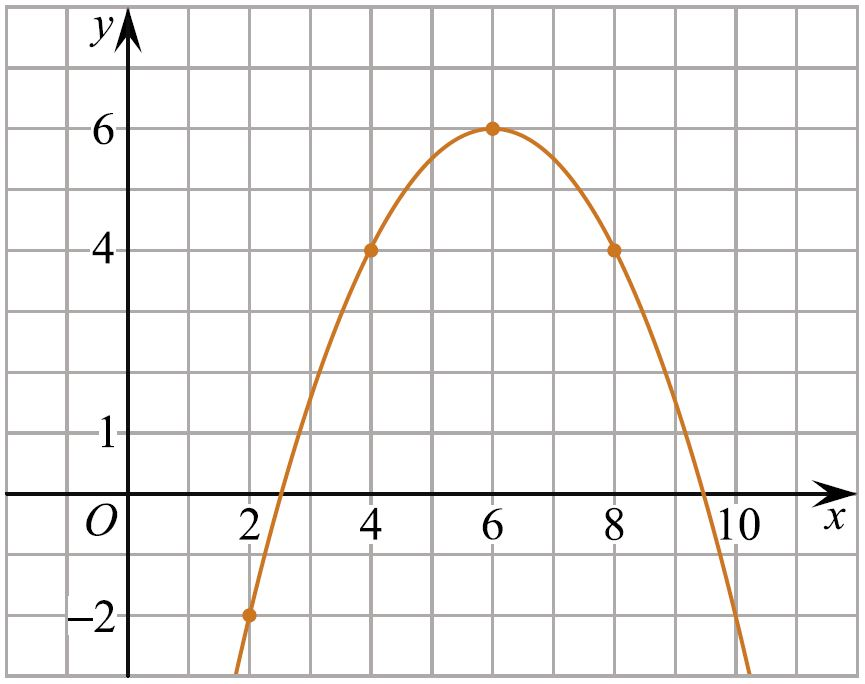
\includegraphics[align=t, width=\linewidth]{../pics/G112M3C1-6}
		%\end{minipage}
		
		
		
		%EGE-1(90g) - 1
		\item В треугольнике \(ABC\) угол \(C\) равен \(90\degree\), \(AC=4,8\), \( \sin A = \dfrac{ 7 }{ 25 } \). Найдите \(AB\).
		%EGE-1(90g) - 4
		\item В треугольнике \(ABC\) угол \(C\) равен \(90\degree\), \(AC=4\), \( \tg A = \dfrac{ 33 }{ 4\sqrt{33} } \). Найдите \(AB\). 
		%n5 cos1
		\item Найдите корни уравнения: \( \cos \dfrac{ \pi(x-7) }{ 3 } = 0,5 \).  В ответ запишите наибольший отрицательный корень.
		%n5 cos3
		\item Найдите корни уравнения: \( \cos \dfrac{ \pi(2x+9) }{ 3 } = \dfrac{ \sqrt{2} }{ 2 } \).  В ответ запишите наибольший отрицательный корень.
		%n5 tg1
		\item Найдите корни уравнения: \( \tg \dfrac{ \pi x }{ 4 } = -1 \).  В ответ запишите наибольший отрицательный корень.
		%n5 tg2
		\item Найдите корни уравнения: \( \tg \dfrac{ \pi (x+2) }{ 3 } = -\sqrt{3} \).  В ответ запишите наибольший отрицательный корень.
		%n5 sin1
		\item Найдите корни уравнения: \( \sin \dfrac{ \pi x }{ 3 } = 0,5 \).  В ответ запишите наименьший положительный корень.
		
		%???chelnokovam5
		\item Вычислить: 
		\begin{tasks}(2)
			\task \( \dfrac{5\cos29\degree}{\sin61\degree} \)
			\task \( -4\sqrt{3}\cos(-750\degree) \)
			\task \( \dfrac{4\cos146\degree}{\cos34\degree} \)
			\task \( 7\tg13\degree\cdot\tg77\degree \)
			\task \( \dfrac{12}{\sin^227\degree+\cos^2207\degree} \)
			\task \( \dfrac{5\sin98\degree}{\sin49\degree\cdot\sin41\degree} \)
			\task \( -50\tg9\degree\cdot\tg81\degree+31 \)
		\end{tasks}
		%?
		\item
		\begin{minipage}[t]{\bodywidth}
			На рисунке изображён график функции \[ f(x)=a \cos{x}+b \] Найдите \(a\).
		\end{minipage}
		\hspace{0.02\linewidth}
		\begin{minipage}[t]{\picwidth}
			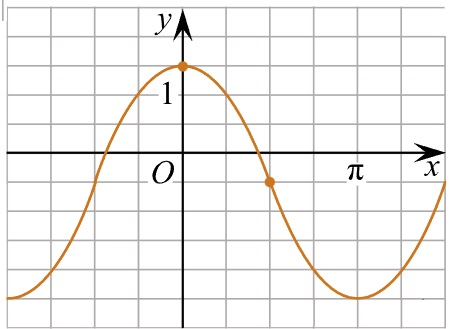
\includegraphics[align=t, width=\linewidth]{\picpath/MECGERM6H3-1}
		\end{minipage}
		%?
		\item
		\begin{minipage}[t]{\bodywidth}
			На рисунке изображён график функции \[ f(x)=a \tg{x}+b \] Найдите \(a\).
		\end{minipage}
		\hspace{0.02\linewidth}
		\begin{minipage}[t]{\picwidth}
			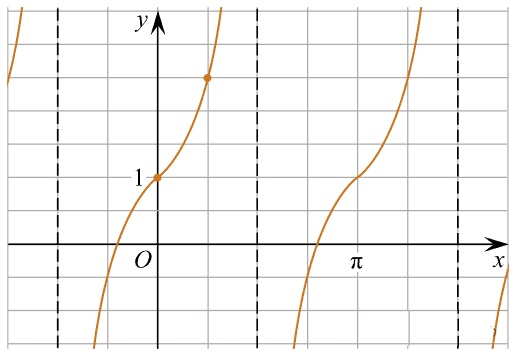
\includegraphics[align=t, width=\linewidth]{\picpath/MECGERM6H3-2}
		\end{minipage}
		%EGE-11 Trigon 1-3
		\item Найдите наибольшее значение функции \[ y=12\cos x + 6\sqrt{3}x - 2 \sqrt{3}x - 2 \sqrt{3} \pi + 6\] на отрезке \( \left[ 0; \dfrac{ \pi }{ 2 } \right]  \).
		\item Найдите наименьшее значение функции \( y=3+\dfrac{ 5\pi }{ 4 }-5x-5\sqrt{2} \cos x\) на отрезке \( \left[ 0; \dfrac{ \pi }{ 2 } \right]  \).
		\item Найдите наибольшее значение функции \( y=5 \cos x - 6x + 4 \) на отрезке \( \left[ -\dfrac{ 3\pi }{ 2 }; 0 \right]  \).
	\end{listofex}
\end{class}
%END_FOLD

%BEGIN_FOLD % ====>>_____ Занятие 2 _____<<====
\begin{class}[number=2]
	\begin{listofex}
		\item Вычислить с помощью метода приведения: %из 101L1
		\[ \cos 225 \degree;\;\sin 420 \degree;\;\sin 270 \degree;\;\sin (-300) ;\;\cos 210 \degree \]
		%;\;\sin\dfrac{13\pi}{4};\;\sin\left( -\dfrac{7\pi}{6}  \right);\;\cos\dfrac{21\pi}{4} 
		\item Вычислите: %из 101L1
		\begin{tasks}(2)
			\task \( \dfrac{\sqrt{3}}{\sin60\degree}+\dfrac{3}{\sin30\degree} \)
			\task \( \dfrac{17\sin155\degree}{\sin25\degree} \)
			\task \( \dfrac{-2\sin105\degree}{\cos15\degree} \)
			\task \( \dfrac{-13\sin126\degree}{\sin54\degree} \)
			\task \( \dfrac{ 8 }{ \sin \left( \tfrac{ -27\pi }{ 4 } \right) \cos \left( \tfrac{ 31\pi }{ 4 } \right) } \)
			\task \( \dfrac{ 60 }{ \sin \left( -\tfrac{ -32\pi }{ 3 } \right) \cos \left( \tfrac{ 25\pi }{ 6 } \right)} \)
			\task \( 4 \sqrt{2} \cos \dfrac{ \pi }{ 4 } \cos \dfrac{ 7\pi }{3  } \)
			\task \( \dfrac{ 5 \cos 29 \degree }{ \sin 61 \degree } \)
			\task \( 36 \sqrt{6} \tg \dfrac{ \pi }{ 6 } \sin \dfrac{ \pi }{ 4 } \)
			\task \( -4 \sqrt{3} \cos (-750 \degree) \)
			
			\task \( \sin^215\degree-1+\cos^215 \degree \)
			\task \( \cos^2\left( -\dfrac{ 3\pi }{ 8 } \right) +\sin^2\left( -\dfrac{ 3\pi }{ 8 } \right) \)
			\task \( \sin^2 (-88\degree) + \cos^2 (-88\degree) -5 \)
			
			\task \( \dfrac{2\sin^221\degree+2\cos^221\degree}{4} \)
			\task \( \dfrac{ 12\sin 11 \degree \cdot \cos 11 \degree }{ \sin 22 \degree } \)
			\task \( \dfrac{ 24 (\sin^2 17 \degree-\cos^217 \degree) }{ \cos 34 \degree } \)
			
			
			
			%\task \( -\sqrt{27}\cos30\degree-\sqrt{2}\sin45\degree\ctg60\degree\tg60\degree\)
		\end{tasks}
		\item Найдите: %101L1
		\begin{tasks}
			
			\task \( 5\sin\alpha \), если \( \cos\alpha=\dfrac{2\sqrt{6}}{5} \) и \( \alpha\in\left( \dfrac{3\pi}{2}; 2\pi \right) \);
			\task \( 3\cos\alpha \), если \( \sin\alpha=-\dfrac{2\sqrt{2}}{3} \) и \( \alpha\in\left( \dfrac{3\pi}{2}; 2\pi \right) \);
			\task \( 24\cos\alpha \), если \( \sin\alpha=-0,2 \);
			\task \( \sin\left( \dfrac{7\pi}{2}-\alpha \right) \), если \( \sin\alpha=0,8 \) и \( \alpha\in\left( \dfrac{\pi}{2}; \pi \right) \).
		\end{tasks}
		%priklad trigon 1
		\item При нормальном падении света с длиной волны \( \lambda=400 \) нм на дифракционную решeтку с периодом \(d\) нм наблюдают серию дифракционных максимумов. При этом угол \(\varphi\)  (отсчитываемый от перпендикуляра к решeтке), под которым наблюдается максимум, и номер максимума \(k\) связаны соотношением \(d \sin \varphi= k\lambda\). Под каким минимальным углом \(\varphi\) (в градусах) можно наблюдать второй максимум на решeтке с периодом, не превосходящим \(1600\) нм?
		%priklad trigon 2
		\item Два тела массой \(m=2\) кг каждое, движутся с одинаковой скоростью  \(v =10\) м/с под углом \(2\alpha\) друг к другу. Энергия (в джоулях), выделяющаяся при их абсолютно неупругом соударении определяется выражением \(Q= m v^2 \sin^2 \alpha \). Под каким наименьшим углом \(2\alpha\) (в градусах) должны двигаться тела, чтобы в результате соударения выделилось не менее \(50\) джоулей?
		\item Найдите площадь треугольника, две стороны которого равны \(8\) и \(12\), а угол между ними равен \(30 \degree\).
		\item Большее основание равнобедренной трапеции равно \(34\). Боковая сторона равна \(14\). Синус острого угла равен \( \dfrac{ 2\sqrt{10}}{ 7 } \). Найдите меньшее основание.
		\item Основания равнобедренной трапеции равны \(7\) и \(51\). Тангенс острого угла равен \( \dfrac{ 5 }{ 11 } \).  Найдите высоту трапеции.
		
	\end{listofex}
\end{class}
%END_FOLD

%BEGIN_FOLD % ====>>_ Домашняя работа 1 _<<====
\begin{homework}[number=1]
	\begin{listofex}
		%\item Решите уравнения: %(1) 1 2 // (2) 1 2
		%\begin{tasks}(2)
		%	\task \( (\tg^2x-1)\sqrt{13\cos x} = 0 \)
		%	\task \( (2\cos^2 x + \sin x - 2)\sqrt{5\tg x}=0 \)
		%	\task \( 2\cos \left( \dfrac{ \pi }{ 2 }-x \right)=\tg x \)
		%	\task \( \cos 2x + \sin^2x=0,75 \)
		%\end{tasks}
		\item Вычислите: %n6 10 11 12 13 14
		\begin{tasks}(2)
			\task \( 24 \sqrt{2} \cos \left( -\dfrac{ \pi }{ 3 } \right) \sin \left( -\dfrac{ \pi }{ 4 } \right)  \)
			\task \( -4 \sqrt{3} \cos \left( -\dfrac{ 3\pi }{ 2 } \right) \cos \left( \dfrac{ \pi}{4  } \right) \)
			\task \( \dfrac{ 14 \sin 19 \degree }{ \sin 341 \degree } \)
			\task \( \dfrac{ 4 \cos 146 \degree }{ \cos 34 \degree } \)
			\task \( \dfrac{ 5 \tg 163 \degree }{ \tg 17 \degree } \)
			\task \( \dfrac{14 \sin 409 \degree  }{ \sin 49 \degree } \)
		\end{tasks}
		\item Найдите корень уравнения:
		\begin{tasks}(2)
			\task \( \sqrt{15-2x}=3 \)
			\task \( \sqrt{-72-17x}=-x \)
			\task \( \sqrt{\dfrac{ 6 }{ 4x-54 }}=\dfrac{ 1 }{ 7 } \)
			\task \( \sqrt{\dfrac{ 2x+5 }{ 3 }}=5 \)
		\end{tasks}
		
		
		\item В треугольнике \(ABC\): \(AC=BC, AB=8, \cos A = 0,5\). Найдите \(AC\).
		
	\end{listofex}
\end{homework}
%END_FOLD

%BEGIN_FOLD % ====>>_____ Занятие 3 _____<<====
\begin{class}[number=3]
	\begin{listofex}
		\item Вычислите:
		\begin{tasks}(2)
			\task \( \dfrac{ 5\sin 98 \degree }{ \sin 49\degree \cdot \sin 41\degree } \)
			\task \( \dfrac{ 5\sin 74 \degree }{ \cos 37 \degree \cdot \cos 53 \degree } \)
			\task \( \dfrac{ 23 }{ \sin^2 56 \degree + 1 + \sin^2 146 \degree } \)
			\task \( -\dfrac{ 4 }{ \sin^2 27 \degree + \sin^2 117 \degree } \)
			\task \( \dfrac{ 50 \sin 19 \degree \cos 19 \degree }{ \sin 38 \degree } \)
			\task \( -\dfrac{ 7 }{ \sin^2 \left( \dfrac{ \pi }{ 15 } \right) + \cos^2 \left( \dfrac{ \pi }{ 15 } \right) } \)
			\task \( 36 \sqrt{6} \tg \dfrac{ \pi }{ 6 } \sin \dfrac{ \pi }{ 4 } \)
			\task \( -4 \sqrt{3} \cos (-750 \degree) \)
			
			\task \( \sin^215\degree-1+\cos^215 \degree \)
			\task \( \cos^2\left( -\dfrac{ 3\pi }{ 8 } \right) +\sin^2\left( -\dfrac{ 3\pi }{ 8 } \right) \)
			\task \( \sin^2 (-88\degree) + \cos^2 (-88\degree) -5 \)
			
			\task \( \dfrac{2\sin^221\degree+2\cos^221\degree}{4} \)
			\task \( \dfrac{ 12\sin 11 \degree \cdot \cos 11 \degree }{ \sin 22 \degree } \)
			\task \( \dfrac{ 24 (\sin^2 17 \degree-\cos^217 \degree) }{ \cos 34 \degree } \)
			
		\end{tasks}
		\item Найдите: %101L1
		\begin{tasks}
			
			\task \( 5\sin\alpha \), если \( \cos\alpha=\dfrac{2\sqrt{6}}{5} \) и \( \alpha\in\left( \dfrac{3\pi}{2}; 2\pi \right) \);
			\task \( 3\cos\alpha \), если \( \sin\alpha=-\dfrac{2\sqrt{2}}{3} \) и \( \alpha\in\left( \dfrac{3\pi}{2}; 2\pi \right) \);
			\task \( 24\cos\alpha \), если \( \sin\alpha=-0,2 \);
			\task \( \sin\left( \dfrac{7\pi}{2}-\alpha \right) \), если \( \sin\alpha=0,8 \) и \( \alpha\in\left( \dfrac{\pi}{2}; \pi \right) \);
			\task \( \tg \alpha \), если \( \cos \alpha = \dfrac{ \sqrt{10} }{ 10 } \) и \( \alpha\in\left( \dfrac{ 3\pi }{ 2 };2\pi \right) \);
			\task \( 26 \cos \left( \dfrac{ 3\pi }{ 2 }+\alpha \right) \), если \( \cos \alpha = \dfrac{ 12 }{ 13 } \) и \( \alpha\in\left( \dfrac{ 3\pi }{ 2 };2\pi \right) \);
			\task \( \dfrac{ 10\sin 6 \alpha }{ 3 \cos 3 \alpha } \), если \( \sin 3 \alpha = 0,6 \).
		\end{tasks}
		%priklad trigon 1
		\item При нормальном падении света с длиной волны \( \lambda=400 \) нм на дифракционную решeтку с периодом \(d\) нм наблюдают серию дифракционных максимумов. При этом угол \(\varphi\)  (отсчитываемый от перпендикуляра к решeтке), под которым наблюдается максимум, и номер максимума \(k\) связаны соотношением \(d \sin \varphi= k\lambda\). Под каким минимальным углом \(\varphi\) (в градусах) можно наблюдать второй максимум на решeтке с периодом, не превосходящим \(1600\) нм?
		%priklad trigon 2
		\item Два тела массой \(m=2\) кг каждое, движутся с одинаковой скоростью  \(v =10\) м/с под углом \(2\alpha\) друг к другу. Энергия (в джоулях), выделяющаяся при их абсолютно неупругом соударении определяется выражением \(Q= m v^2 \sin^2 \alpha \). Под каким наименьшим углом \(2\alpha\) (в градусах) должны двигаться тела, чтобы в результате соударения выделилось не менее \(50\) джоулей?
		%priklad trigon 3
		\item Катер должен пересечь реку шириной \(L = 100\) м и со скоростью течения \(u =0,5\) м/с так, чтобы причалить точно напротив места отправления. Он может двигаться с разными скоростями, при этом время в пути, измеряемое в секундах, определяется выражением \(t = \dfrac{ L }{ u } \ctg \alpha \),  где \(\alpha\) --- острый угол, задающий направление его движения (отсчитывается от берега). Под каким минимальным углом \(\alpha\) (в градусах) нужно плыть, чтобы время в пути было не больше \(200\) с?
		\item Найдите площадь треугольника, две стороны которого равны \(8\) и \(12\), а угол между ними равен \(30 \degree\).
		\item Большее основание равнобедренной трапеции равно \(34\). Боковая сторона равна \(14\). Синус острого угла равен \( \dfrac{ 2\sqrt{10}}{ 7 } \). Найдите меньшее основание.
		\item Основания равнобедренной трапеции равны \(7\) и \(51\). Тангенс острого угла равен \( \dfrac{ 5 }{ 11 } \).  Найдите высоту трапеции.
		\item В треугольнике \(ABC\): \(AC=BC=7, \tg A = \dfrac{ 33 }{ 4\sqrt{3} }\). Найдите \(AB\).
	\end{listofex}
\end{class}
%END_FOLD

%BEGIN_FOLD % ====>>_____ Занятие 4 _____<<====
\begin{class}[number=4]
	\begin{listofex}
		\item Найдите:
		\begin{tasks}(2)
			\task \( \dfrac{ \cos 100 \degree }{ 5\sin 50 \degree \cos 50 \degree } \)
			\task \( -\dfrac{ 4\cos 22,5 \degree \sin 22,5 \degree }{ 8 } \)
			\task \( \dfrac{ 50 \sin 19 \degree \cos 19 \degree }{ \sin 38 \degree } \)
			\task \( \dfrac{ \sin \dfrac{ 3\pi }{8 } \cos \dfrac{ 3\pi }{ 8 } }{ 20 } \)
			\task \( \sqrt{50} \cos^2 \dfrac{ 9\pi }{ 8 } - \sqrt{50} \sin^2 \dfrac{ 9\pi }{ 8 } \)
			\task \( 4\sqrt{2} \cos^2 \dfrac{ 15\pi }{ 8 } -2\sqrt{2} \)
		\end{tasks}
		\item Найдите: %последние 5
		\begin{tasks}(1)
			
			\task \(\sin 2 \alpha \), если \( \cos \alpha = 0,6 \) и \( \pi < \alpha < 2 \pi \);
			\task \( \cos \alpha \), если \( \sin \alpha = \dfrac{ 2 \sqrt{6} }{ 5 } \) и \( \alpha \in \left( \dfrac{ \pi }{ 2 }; \pi \right) \);
			\task \( 2\cos 2 \alpha \), если \( \sin \alpha=-0,7 \);
			
			
		\end{tasks}
		
		%priklad trigon 4
		\item Скейтбордист прыгает на стоящую на рельсах платформу, со скоростью  \(v = 3\) м/с под острым углом \(\alpha\)  к рельсам. От толчка платформа начинает ехать со скоростью \(u = \dfrac{ m }{ m+M }v \cos \alpha\) (м/с), где \(m = 80\) кг --- масса скейтбордиста со скейтом, а \(M = 400\) кг --- масса платформы. Под каким максимальным углом \(\alpha\) (в градусах) нужно прыгать, чтобы разогнать платформу не менее чем до \(0,25\) м/с?
		%priklad trigon 5
		\item Груз массой \(0,08\) кг колеблется на пружине. Его скорость υ меняется по закону \( v = v_0 \sin \dfrac{ 2\pi t }{ T } \), где \(t\) --- время с момента начала колебаний, \(T  =  12\) с --- период колебаний, \(v _0=0,5\) м/с. Кинетическая энергия\(E\) (в джоулях) груза вычисляется по формуле \( E = \dfrac{ m v^2 }{ 2 } \),  где \(m\) --- масса груза в килограммах, \(v\) --- скорость груза в м/с. Найдите кинетическую энергию груза через \(1\) секунду после начала колебаний. Ответ дайте в джоулях.
		\item В параллелограмме \(ABCD\) \(AB  = 6, AD  =  42\), \(\sin A= \dfrac{ 6 }{ 7 } \).  Найдите большую высоту параллелограмма.
		\item Найдите площадь ромба, если его высота равна \(2\), а острый угол \(30 \degree \).
		\item Основания равнобедренной трапеции равны \(17\) и \(87\). Высота трапеции равна \(14\). Найдите тангенс острого угла.
		\item Найдите площадь прямоугольной трапеции, основания которой равны \(6\) и \(2\), большая боковая сторона составляет с основанием угол \(45\degree \).
		\item Основания прямоугольной трапеции равны \(12\) и \(4\). Ее площадь равна \(64\). Найдите острый угол этой трапеции. Ответ дайте в градусах.
		\item В треугольнике \(ABC\) \( \angle C = 90 \degree, \tg A = \dfrac{  1}{ 5 } \).  Найдите \(AH\).
		\item В треугольнике \(ABC\) \(\angle C = 90 \degree\). \(CH\) --- высота, \(AB=13, \tg A = 5\). Найдите \(BH\).
	\end{listofex}
\end{class}
%END_FOLD

%BEGIN_FOLD % ====>>_ Домашняя работа 2 _<<====
\begin{homework}[number=2]
	\begin{listofex}
		\item Вычислите:
		\begin{tasks}(2)
			\task \( \dfrac{ 11\cos 150 \degree }{ 3\cos 75 \degree \sin 75 \degree } \)
			\task \( - \cos \left( \dfrac{ 3\pi }{ 8 }  \right) \sin \left( \dfrac{ 3\pi }{ 8 } \right) \)
			\task \( -\sqrt{2} \sin^2 \dfrac{ 2\pi }{ 7 } - \sqrt{2} \cos^2 \dfrac{ 2\pi }{ 7 }  \)
			\task \( 23 \cdot(-5 \sin 54 \degree - 5 \cos 54 \degree) \)
		\end{tasks}
		\item Найдите: %8-10
		\begin{tasks}
			\task \( \sin \left( \dfrac{ 7\pi }{2  }-\alpha \right) \), если \( \sin \alpha = 0,8 \) и \( \alpha \in \left( \dfrac{ \pi }{ 2 }; \pi \right) \);
			\task \( 26 \cos \left( \dfrac{ 3\pi }{ 2 }+\alpha \right) \), если \( \cos \alpha = \dfrac{ 12 }{ 13 } \) и \( \alpha \in \left( \dfrac{ 3\pi }{ 2 }; 2 \pi \right) \).
			%\task \( \tg \left( \alpha+\dfrac{ 5\pi }{ 2 } \right) \), если \( \tg \alpha = 0,4 \).
		\end{tasks}
		%priklad trigon 7
		\item Скорость колеблющегося на пружине груза меняется по закону \(v(5) = 5 \sin \pi t\) (см/с), где \(t\) --- время в секундах. Какую долю времени из первой секунды скорость движения была не менее \(2,5\) см/с? Ответ выразите десятичной дробью, если нужно, округлите до сотых.

	\end{listofex}
\end{homework}
%END_FOLD

%BEGIN_FOLD % ====>>_____ Занятие 5 _____<<====
\begin{class}[number=5]
	\begin{listofex}
		%\item
		%\begin{minipage}[t]{\bodywidth}
		%	На рисунке изображен график функции \( f(x)=kx+b \). Найдите \( f(-9) \).
		%\end{minipage}
		%\begin{minipage}[t]{\picwidth}
		%	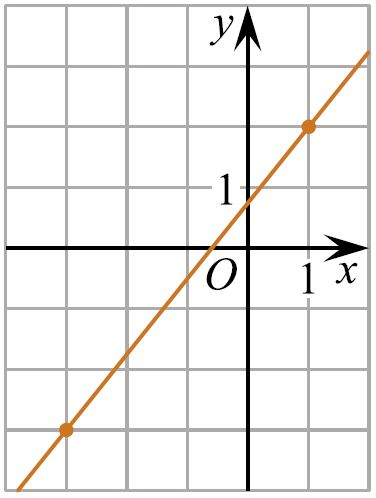
\includegraphics[align=t, width=0.8\textwidth]{\picpath/G112M3C2-1}
		%\end{minipage}
		\item 
		\begin{minipage}[t]{\bodywidth}
				На рисунке изображён график функции \(f(x)=kx+b\). Найдите \(f(-5)\).
			\end{minipage}
		\begin{minipage}[t]{\picwidth}
				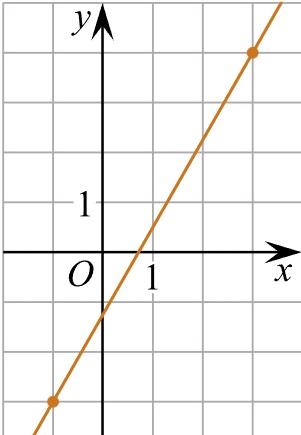
\includegraphics[align=t, width=0.8\textwidth]{\picpath/G101M4H2-1.jpg}
			\end{minipage}
		\item
		\begin{minipage}[t]{\bodywidth}
			На рисунке изображены графики двух линейных функций. Найдите абсциссу точки пересечения графиков.
		\end{minipage}
		\begin{minipage}[t]{\picwidth}
			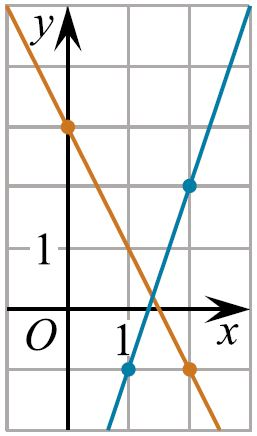
\includegraphics[align=t, width=0.8\textwidth]{\picpath/G112M3C2-2}
		\end{minipage}
		\item
	\begin{minipage}[t]{\bodywidth}
			На рисунке изображён график функции вида \(f(x)=ax^2+bx+c\), где числа \(a, b, c\) --- целые. Найдите значение \(f(-3)\).
		\end{minipage}
	\begin{minipage}[t]{\picwidth}
			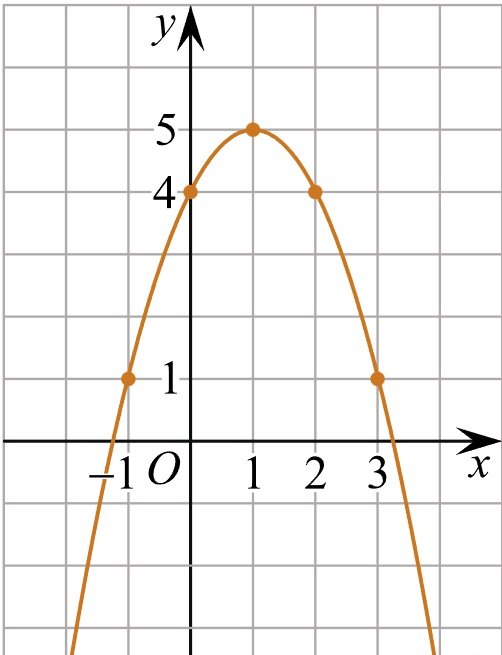
\includegraphics[align=t, width=\textwidth]{\picpath/G101M4C4-3.jpg}
		\end{minipage}
		
		\item
		\begin{minipage}[t]{\bodywidth}
			На рисунке изображен график функции \( f(x)=\dfrac{x^2}{a}+bx+c \). Найдите \( f(3,5) \).
		\end{minipage}
		\begin{minipage}[t]{\picwidth}
			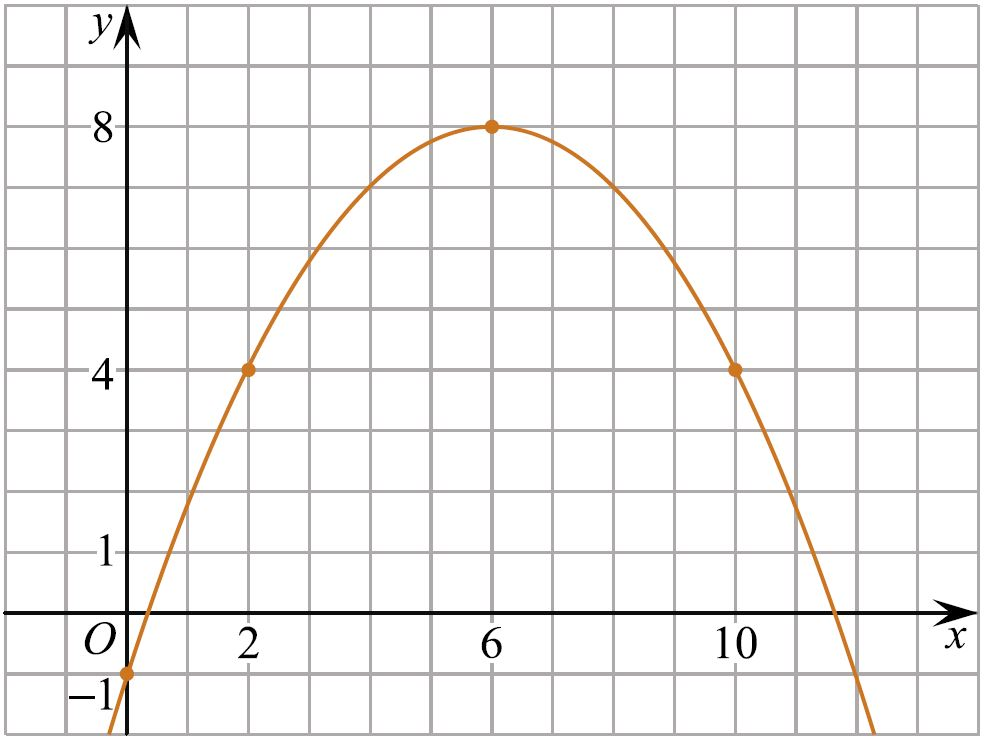
\includegraphics[align=t, width=\textwidth]{\picpath/G112M3C2-3}
		\end{minipage}
		
		\item
	\begin{minipage}[t]{\bodywidth}
			На рисунке изображён график функции вида \(f(x)=ax^2+bx+c\), где числа \(a, b, c\) --- целые. Найдите значение дискриминанта уравнения \(f(x)=0\).
		\end{minipage}
	\begin{minipage}[t]{\picwidth}
			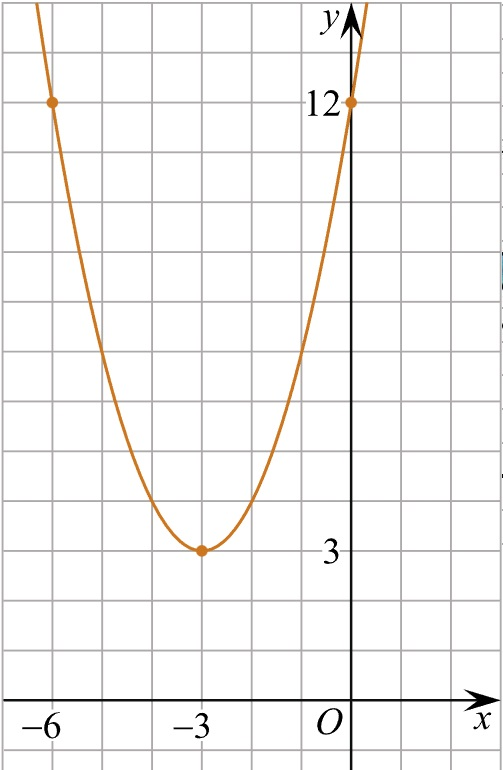
\includegraphics[align=t, width=\textwidth]{\picpath/G101M4C4-5.jpg}
		\end{minipage}
		
		\item
		\begin{minipage}[t]{\bodywidth}
			На рисунке изображены графики функций \( f(x)=2x^2+11x+11 \) и \( y=ax^2+bx+c \), которые пересекаются в точках \( A \) и \( B \). Найдите абсциссу точки \( B \).
		\end{minipage}
		\begin{minipage}[t]{\picwidth}
			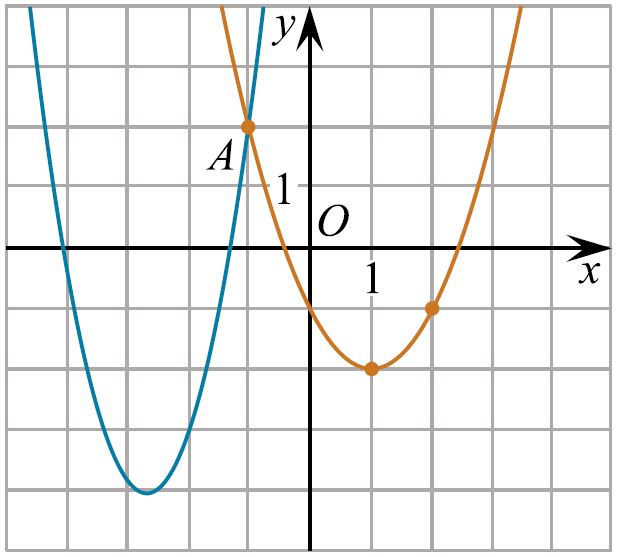
\includegraphics[align=t, width=\textwidth]{\picpath/G112M3C2-6}
		\end{minipage}
			\item
		\begin{minipage}[t]{\bodywidth}
			На рисунке изображен график функции \( f(x)=\dfrac{k}{x}+a \). Найдите, при каком значении \( x \) значение функции будет равно \( 0,8 \).
		\end{minipage}
		\begin{minipage}[t]{\picwidth}
			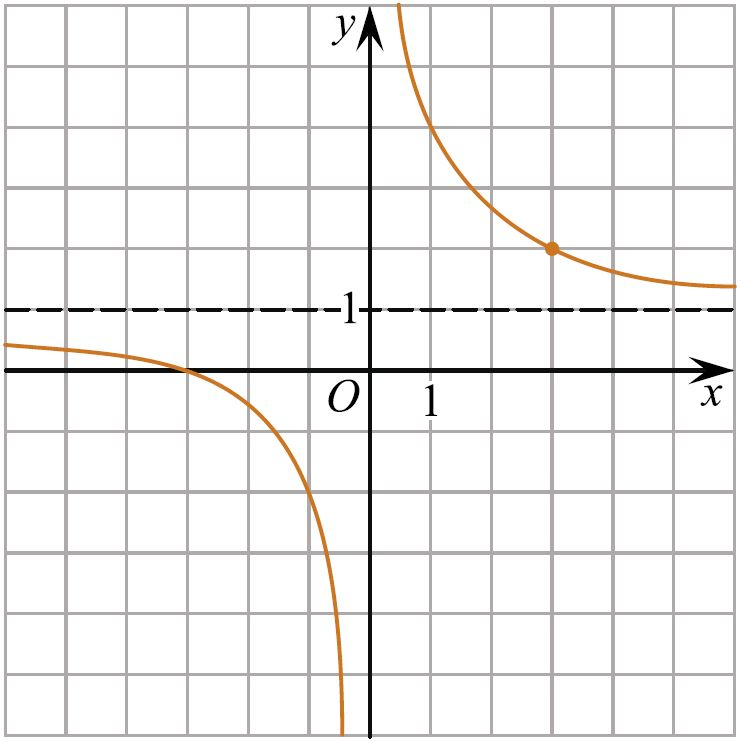
\includegraphics[align=t, width=\textwidth]{\picpath/G112M3C2-5}
		\end{minipage}
		\item
		\begin{minipage}[t]{\bodywidth}
			На рисунке изображён график функции вида \[ f(x)=\dfrac{a}{x+b}+c, \] где числа \(a, b, c\) --- целые. Найдите значение \(x\), при котором \(f(x)=3\).
		\end{minipage}
		\hspace{0.02\linewidth}
		\begin{minipage}[t]{\picwidth}
			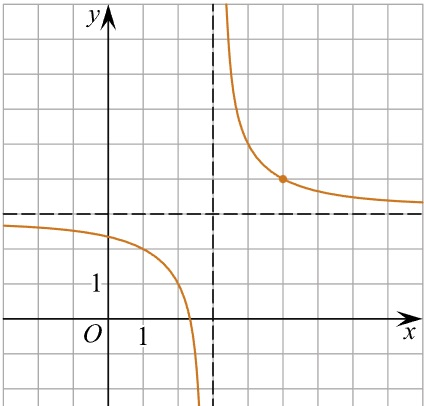
\includegraphics[align=t, width=\linewidth]{\picpath/G101M4C6-2}
		\end{minipage}
		\newpage
		%analog 26784 1-2 V 62785 1-2
		\item Найдите:
		\begin{tasks}
			\task \( 8 \sin \left( \dfrac{ \pi }{ 2 }- \alpha \right) \), если \( \sin \alpha = -0,6 \) и \( \alpha \in (1,5\pi;2\pi) \);
			\task \( -2 \sin \left( \dfrac{ \pi }{ 2 }+\alpha \right) \), если \( \sin \alpha = -0,96 \) и \( \alpha \in (\pi;1,5\pi) \);
			\task \( -20 \cos \left( \dfrac{ 5\pi }{ 2 }+ \alpha \right) \), если \( \cos \alpha = \dfrac{ 7 }{ 25 } \) и \( \alpha \in (1,5\pi; 2\pi) \);
			\task \( 39 \cos \left( \dfrac{ 7\pi }{ 2 } + \alpha \right) \), если \( \cos \alpha = -\dfrac{ 7\pi }{ 2 } + \alpha \) и \( \alpha \in (0,5\pi;\pi) \).
		\end{tasks}
		\item Вычислите:
		\begin{tasks}(2)
			\task \( \dfrac{ 36 \sin 102 \degree \cdot \cos 102 \degree }{ \sin 204 \degree } \)
			\task \( \dfrac{ 50 \sin 38 \degree }{ \sin 19 \degree \cdot \cos 19 \degree } \)
			\task \( \dfrac{ -10 \sin 97 \degree \cdot \cos 97 \degree }{ \sin 194 \degree } \)
			\task \( \dfrac{ -16 \sin 112 \degree \cdot \cos 112 \degree }{ 5 \sin 224 \degree } \)
			\task \( \dfrac{22 (\sin^2 72 \degree - \cos^2 72 \degree)}{ \cos 144 \degree } \)
			\task \( \dfrac{ 22 \cos 18 \degree }{ \sin^2 9 \degree - \cos^2 9 \degree  } \)
			\task \( \dfrac{ 18(-\sin^2 24 \degree + \cos^2 24 \degree) }{ \cos 48 \degree } \)
			\task \( \dfrac{ 7(\sin^2 11 \degree - \cos^2 11 \degree) }{ -\cos 22 \degree } \)
		\end{tasks}
	\end{listofex}
\end{class}
%END_FOLD

%BEGIN_FOLD % ====>>_____ Занятие 6 _____<<====
\begin{class}[number=6]
	\begin{listofex}
		\item
		\begin{minipage}[t]{\bodywidth}
			На рисунке изображен график функции \( f(x)=\dfrac{x^2}{a}+bx+c \). Найдите \( f(4) \).
		\end{minipage}
		\begin{minipage}[t]{\picwidth}
			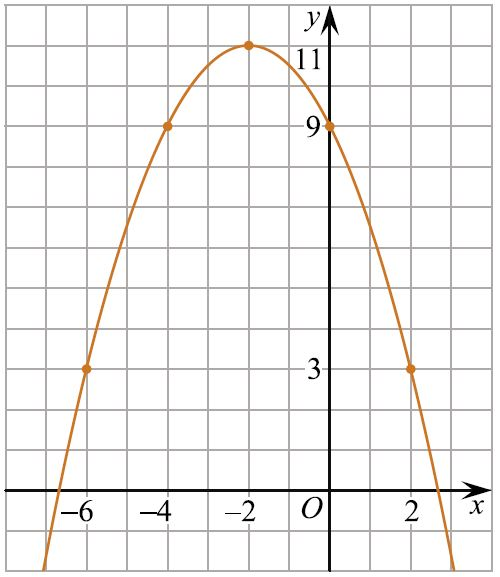
\includegraphics[align=t, width=\textwidth]{\picpath/G112M3C2-4}
		\end{minipage}
		\item
		\begin{minipage}[t]{\bodywidth}
			На рисунке изображён график функции вида \(f(x)= \log_ax\). Найдите значение \(f(8)\).
		\end{minipage}
		\begin{minipage}[t]{\picwidth}
			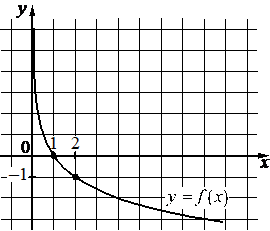
\includegraphics[align=t, width=\textwidth]{\picpath/G111M8L6-1}
		\end{minipage}
		\item
		\begin{minipage}[t]{\bodywidth}
			На рисунке изображён график функции вида \(f(x)= \log_a x\). Найдите значение \(f(8)\).
		\end{minipage}
		\begin{minipage}[t]{\picwidth}
			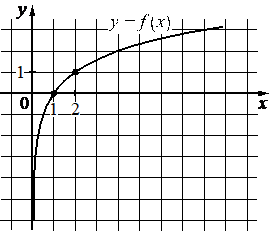
\includegraphics[align=t, width=\textwidth]{\picpath/G111M8L6-4}
		\end{minipage}
		\item
		\begin{minipage}[t]{\bodywidth}
			На рисунке изображён график функции вида \(f(x)= \log_ax\). Найдите значение \(f(2)\).
		\end{minipage}
		\begin{minipage}[t]{\picwidth}
			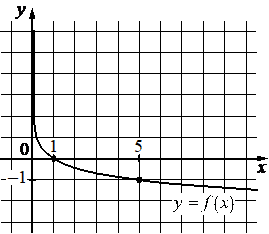
\includegraphics[align=t, width=\textwidth]{\picpath/G111M8L6-8}
		\end{minipage}
		\item
		\begin{minipage}[t]{\bodywidth}
			На рисунке изображён график функции вида \(f(x)= a^x\). Найдите значение \(f(3)\).
		\end{minipage}
		\begin{minipage}[t]{\picwidth}
			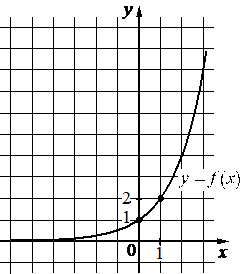
\includegraphics[align=t, width=\textwidth]{\picpath/G111M8L6-2}
		\end{minipage}
		\item
		\begin{minipage}[t]{\bodywidth}
			На рисунке изображён график функции вида \(f(x)= a^x\). Найдите значение \(f(-3)\).
		\end{minipage}
		\begin{minipage}[t]{\picwidth}
			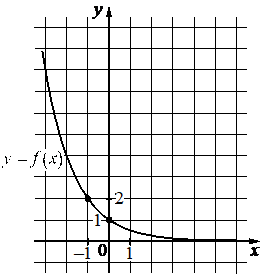
\includegraphics[align=t, width=\textwidth]{\picpath/G111M8L6-3}
		\end{minipage}
		
		\item
		\begin{minipage}[t]{\bodywidth}
			На рисунке изображён график функции вида \(f(x)= a^x\). Найдите значение \(f(4)\).
		\end{minipage}
		\begin{minipage}[t]{\picwidth}
			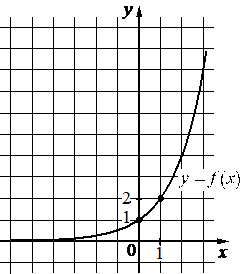
\includegraphics[align=t, width=\textwidth]{\picpath/G111M8L6-5}
		\end{minipage}
		
		\item
		\begin{minipage}[t]{\bodywidth}
			На рисунке изображён график функции вида \(f(x)= a^x\). Найдите значение \(f(2)\).
		\end{minipage}
		\begin{minipage}[t]{\picwidth}
			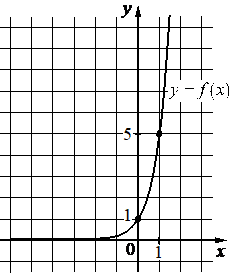
\includegraphics[align=t, width=\textwidth]{\picpath/G111M8L6-7}
		\end{minipage}
		
		\item
		\begin{minipage}[t]{\bodywidth}
			На рисунке изображены графики функций видов \(f(x)= a\sqrt{x} \) и  \(g(x)=kx\), пересекающиеся в точках \(A\) и \(B\). Найдите абсциссу точки \(B\).
		\end{minipage}
		\begin{minipage}[t]{\picwidth}
			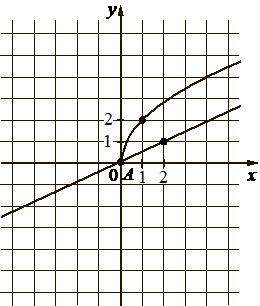
\includegraphics[align=t, width=\textwidth]{\picpath/G111M8L6-6}
		\end{minipage}
		%priklad POKAZ 1
		\item При адиабатическом процессе для идеального газа выполняется закон \(pV^k=10^5\)Па\(\cdot\)м\(^5\), где \(p\) --- давление газа в паскалях, \(V\) --- объeм газа в кубических метрах, \(k=\dfrac{  5}{ 3 }\).  Найдите, какой объём \(V\) (в куб. м) будет занимать газ при давлении \(p\), равном \(3,2\cdot10^6\) Па.
		%priklad POKAZ 2
		\item В ходе распада радиоактивного изотопа его масса уменьшается по закону \( m(t)=m_02^{-\tfrac{ t }{ T }} \), где \(m_0\) --- начальная масса изотопа, \(t\) --- время, прошедшее от начального момента, \(T\) --- период полураспада. В начальный момент времени масса изотопа \(40\) мг. Период его полураспада составляет \(10\) мин. Найдите, через сколько минут масса изотопа будет равна \(5\) мг.
	\end{listofex}
\end{class}
%END_FOLD

%BEGIN_FOLD % ====>>_ Домашняя работа 3 _<<====
\begin{homework}[number=3]
	\begin{listofex}
		\item Вычислите: %первые 4
		\begin{tasks}(2)
			\task \( 6^{0,36}\cdot 36^{0,32} \)
			\task \( 7^{\tfrac{ 4 }{ 9 }} \cdot 49^{\tfrac{ 5 }{ 18 }} \)
			\task \( \dfrac{ 5^{6,5} }{ 25^{2,25} } \)
			\task \( \dfrac{  2^{3,5}\cdot 3^{5,5}}{ 6^{4,5} } \)
		\end{tasks}
		\item Найдите значение выражений: %первые 4
		\begin{tasks}(2)
			\task \( \dfrac{ 7(m^5)^6+11(m^3)^{10} }{ (3m^{15})^2 } \)
			\task \( \dfrac{ (3x)^3\cdot x^{-9} }{ x^{-10}\cdot2x^4 } \)
			\task \( \dfrac{ a^2b^{-6} }{ (4a)^3b^{-2} }\cdot \dfrac{ 16 }{ a^{-1} b^{-4}} \)
			\task \( ((2x^3)^4-(x^2)^6):(3x^{12}) \)
		\end{tasks}
		\item При адиабатическом процессе для идеального газа выполняется закон \(pV^k=1,25 \cdot 10^8\)Па\(\cdot\)м\(^4\), где \(p\) --- давление газа в паскалях, \(V\) --- объeм газа в кубических метрах, \(k=\dfrac{  4}{ 3 }\).  Найдите, какой объём \(V\) (в куб. м) будет занимать газ при давлении \(p\), равном \(2\cdot10^5\) Па.
		\item
		\begin{minipage}[t]{0.65\linewidth}
			На рисунке изображены графики функций \(f(x)=a\sqrt{x} \) и \(g(x)=kx+b\), которые пересекаются в точке \(A\). Найдите абсциссу точки \(A\).
		\end{minipage}
		\begin{minipage}[t]{0.32\linewidth}
			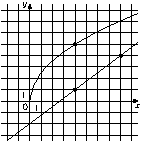
\includegraphics[align=t, width=\textwidth]{\picpath/G111M8H3-3}
		\end{minipage}
		\item
		\begin{minipage}[t]{0.65\linewidth}
			На рисунке изображены графики функций \(f(x)=-3x+13\) и \(g(x)=ax^2+bx+c\), которые пересекаются в точках \(A\) и \(B\). Найдите абсциссу точки \(B\).
		\end{minipage}
		\begin{minipage}[t]{0.32\linewidth}
			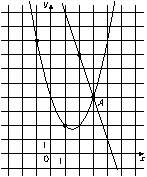
\includegraphics[align=t, width=\textwidth]{\picpath/G111M8H3-2}
		\end{minipage}
		\item
		\begin{minipage}[t]{0.65\linewidth}
			На рисунке изображён график функции \(f(x)=\log_{a}(x+b)\). Найдите \(f(29)\).
		\end{minipage}
		\begin{minipage}[t]{0.32\linewidth}
			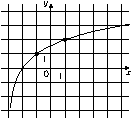
\includegraphics[align=t, width=\textwidth]{\picpath/G111M8H3-4}
		\end{minipage}
		%\item
		%\begin{minipage}[t]{0.65\linewidth}
		%	На рисунке изображён график функции \(f(x)=\dfrac{ kx+a }{ x+b }\). Найдите \(a\).
		%\end{minipage}
		%\begin{minipage}[t]{0.32\linewidth}
		%	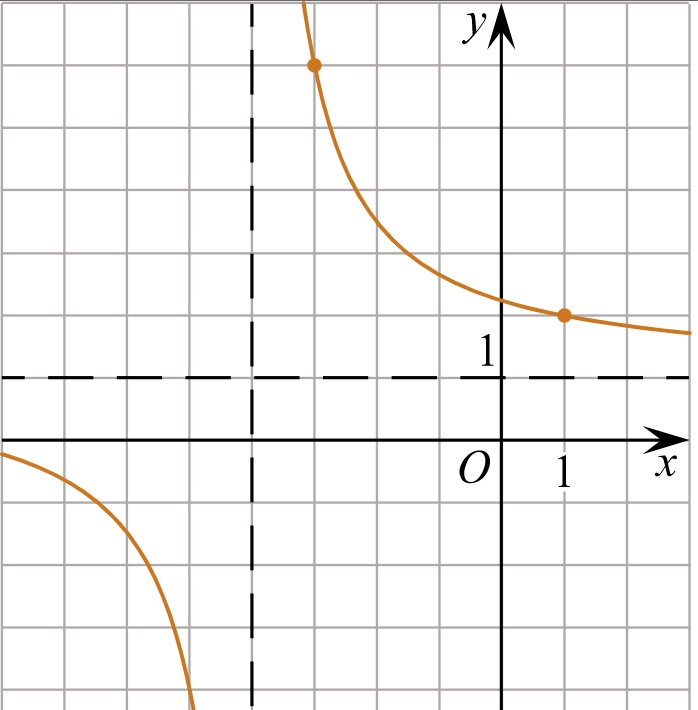
\includegraphics[align=t, width=\textwidth]{\picpath/G111M8H3-1}
		%\end{minipage}
		\item
		\begin{minipage}[t]{0.63\linewidth}
			На рисунке изображен график функции \(f(x)=\dfrac{ k }{ x+a }\). Найдите значение \(x\), при котором \(f(x)=0,2\).
		\end{minipage}
		\hspace{0.02\linewidth}
		\begin{minipage}[t]{0.32\linewidth}
			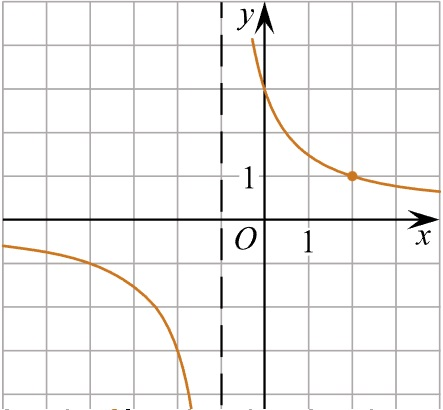
\includegraphics[align=t, width=\linewidth]{../pics/G112M8H3-2}
		\end{minipage}
	\end{listofex}
\end{homework}
%END_FOLD

%BEGIN_FOLD % ====>>_____ Занятие 7 _____<<====
\begin{class}[number=7]
	\begin{listofex}
		\item
		\begin{minipage}[t]{\bodywidth}
			На рисунке изображён график функции \(f(x)=2x^2+bx+c\). Найдите значение \(f(-3)\).
		\end{minipage}
		\begin{minipage}[t]{\picwidth}
			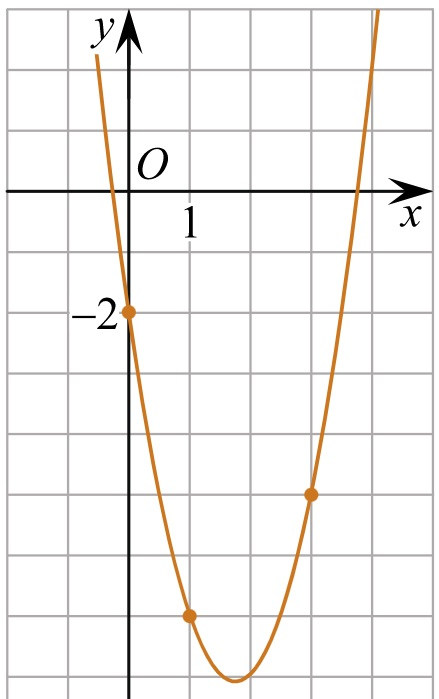
\includegraphics[align=t, width=\textwidth]{\picpath/G111M8L7-1}
		\end{minipage}
		\item
		\begin{minipage}[t]{0.6\linewidth}
			На рисунке изображён график функции \(f(x)=\dfrac{k}{x} +a\). Найдите \(f(7,5)\).
		\end{minipage}
		\begin{minipage}[t]{0.35\linewidth}
			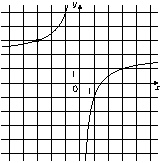
\includegraphics[align=t, width=\textwidth]{\picpath/G111M8L7-2}
		\end{minipage}
		\item
		\begin{minipage}[t]{0.6\linewidth}
			На рисунке изображён график функции \(f(x)=a^x+b\). Найдите значение \(x\), при котором \(f(x)=29\).
		\end{minipage}
		\begin{minipage}[t]{0.35\linewidth}
			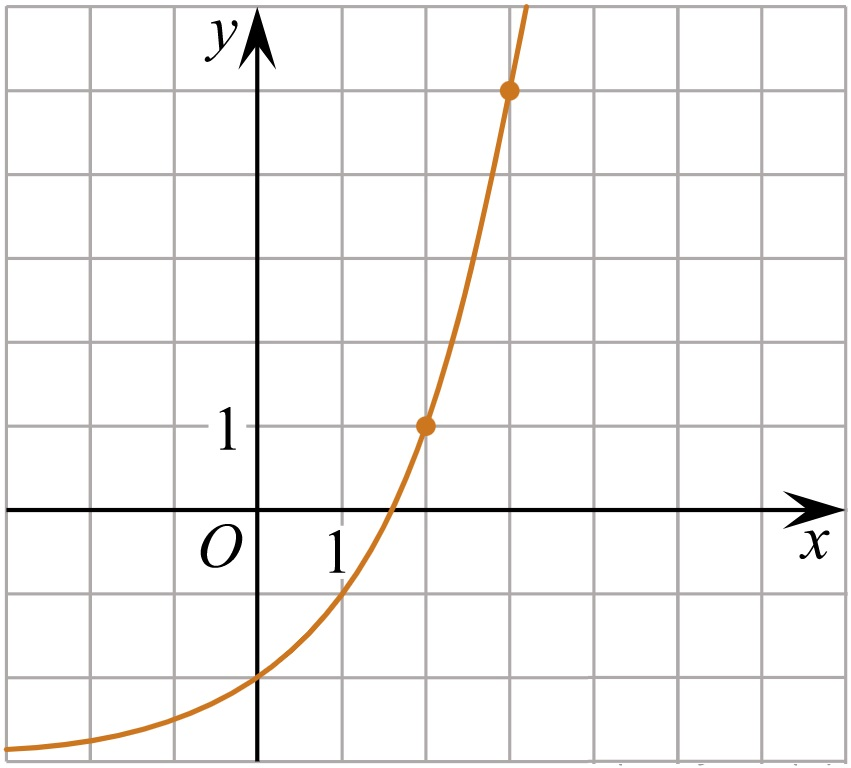
\includegraphics[align=t, width=\textwidth]{\picpath/G111M8L7-3}
		\end{minipage}
		\item
		\begin{minipage}[t]{0.6\linewidth}
			На рисунке изображён график функции \(f(x)=b+\log_{a} x\). Найдите \(f(16)\).
		\end{minipage}
		\begin{minipage}[t]{0.35\linewidth}
			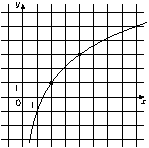
\includegraphics[align=t, width=\textwidth]{\picpath/G111M8L7-4}
		\end{minipage}
		\item
		\begin{minipage}[t]{0.56\linewidth}
			На рисунке изображён график функции \(f(x)=a\cos x + b\). Найдите \(a\).
		\end{minipage}
		\begin{minipage}[t]{0.4\linewidth}
			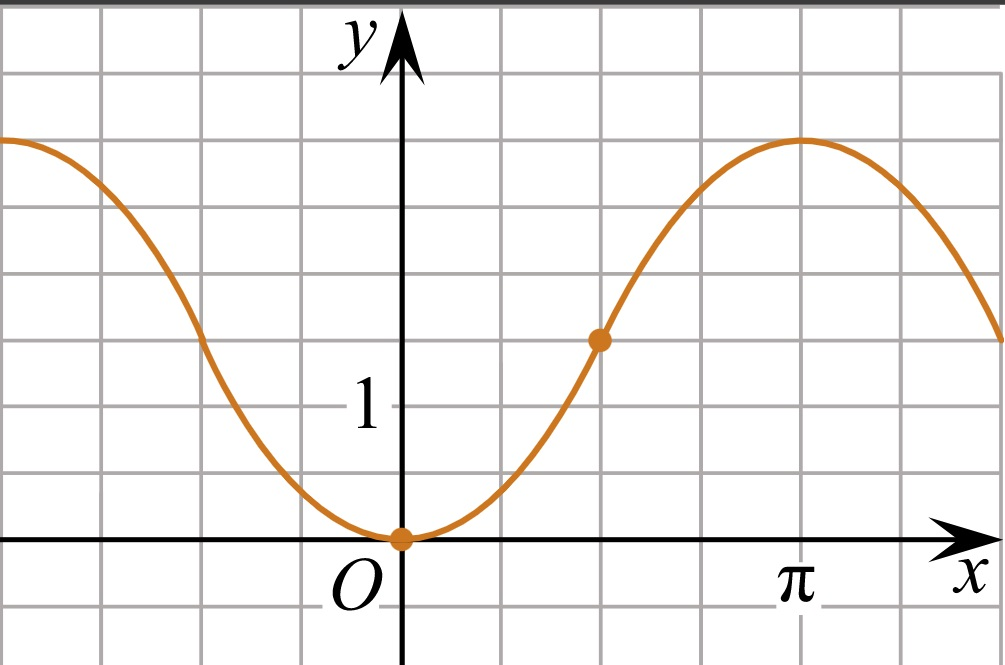
\includegraphics[align=t, width=\textwidth]{\picpath/G111M8L7-5}
		\end{minipage}
		%priamaia 5, krug 5, rabota 5
		\item Велосипедист выехал с постоянной скоростью из города \(A\) в город \(B\), расстояние между которыми равно \(98\) км. На следующий день он отправился обратно со скоростью на \(7\) км/ч больше прежней. По дороге он сделал остановку на \(7\) часов. В результате он затратил на обратный путь столько же времени, сколько на путь из \(A\) в \(B\). Найдите скорость велосипедиста на пути из \(A\) в \(B\). Ответ дайте в км/ч.
		\item Моторная лодка прошла против течения реки \(112\) км и вернулась в пункт отправления, затратив на обратный путь на \(6\) часов меньше. Найдите скорость течения, если скорость лодки в неподвижной воде равна \(11\) км/ч. Ответ дайте в км/ч.
		\item На изготовление \(475\) деталей первый рабочий тратит на \(6\) часов меньше, чем второй рабочий на изготовление \(550\) таких же деталей. Известно, что первый рабочий за час делает на \(3\) детали больше, чем второй. Сколько деталей в час делает первый рабочий?
		\item Первая труба пропускает на \(3\) литра воды в минуту меньше, чем вторая. Сколько литров воды в минуту пропускает первая труба, если резервуар объемом \(108\) литров она заполняет на \(3\) минуты дольше, чем вторая труба?
		\item Два тела массой \(m=2\) кг каждое, движутся с одинаковой скоростью  \(v =10\) м/с под углом \(2\alpha\) друг к другу. Энергия (в джоулях), выделяющаяся при их абсолютно неупругом соударении определяется выражением \(Q = m v^2\sin^2 \alpha \). Под каким наименьшим углом \(2\alpha\) (в градусах) должны двигаться тела, чтобы в результате соударения выделилось не менее \(50\) джоулей?
		\item По закону Ома для полной цепи сила тока, измеряемая в амперах, равна \( I=\dfrac{ \varepsilon }{ R+r } \), где \(\varepsilon\) --- ЭДС источника (в вольтах), \(r=1\) Ом --- его внутреннее сопротивление, \(R\) --- сопротивление цепи (в омах). При каком наименьшем сопротивлении цепи сила тока будет составлять не более \(20\%\) от силы тока короткого замыкания \(I_{kz}=\dfrac{ \varepsilon }{ r }\). (Ответ выразите в омах.)
		%\item Два гонщика участвуют в гонках. Им предстоит проехать \(60\) кругов по кольцевой трассе протяжённостью \(3\) км. Оба гонщика стартовали одновременно, а на финиш первый пришёл раньше второго на \(10\) минут. Чему равнялась средняя скорость второго гонщика, если известно, что первый гонщик в первый раз обогнал второго на круг через \(15\) минут? Ответ дайте в км/ч.
		%\item Двое рабочих, работая вместе, могут выполнить работу за \(12\) дней. За сколько дней, работая отдельно, выполнит эту работу первый рабочий, если он за два дня выполняет такую же часть работы, какую второй --- за три дня?
	\end{listofex}
\end{class}
%END_FOLD

%BEGIN_FOLD % ====>>_ Проверочная работа _<<====
\begin{class}[number=8]
	\begin{listofex}
		%20.4 n1,3,5,14
		\item Плот и лодка движутся навстречу друг другу по реке. Они находятся на расстоянии \(20\) км друг от друга. Через какое время они встретятся, если собственная скорость лодки \(8\) км/ч, а скорость течения реки \(2\) км/ч?
		\item Моторная лодка прошла против течения реки \(112\) км и вернулась в пункт отправления, затратив на обратный путь на \(6\) часов меньше. Найдите скорость течения, если скорость лодки в неподвижной воде равна \(11\) км/ч. Ответ дайте в км/ч.
		\item Моторная лодка в \(10:00\) вышла из пункта \(A\) в пункт \(B\), расположенный в \(30\) км от \(A\). Пробыв в пункте \(B\) \(2\) часа \(30\) минут, лодка отправилась назад и вернулась в пункт \(A\) в \(18:00\). Определите (в км/ч) собственную скорость лодки, если известно, что скорость течения реки \(1\) км/ч.
		\item Теплоход проходит по течению реки до пункта назначения \(255\) км и после стоянки возвращается в пункт отправления. Найдите скорость теплохода в неподвижной воде, если скорость течения равна \(1\) км/ч, стоянка длится \(2\) часа, а в пункт отправления теплоход возвращается через \(34\) часа после отплытия из него. Ответ дайте в км/ч.
		\item Теплоход проходит по течению реки до пункта назначения \(200\) км и после стоянки возвращается в пункт отправления. Найдите скорость течения, если скорость теплохода в неподвижной воде равна \(15\) км/ч, стоянка длится \(10\) часов, а в пункт отправления теплоход возвращается через \(40\) часов после отплытия из него. Ответ дайте в км/ч.
		%\item Весной катер идёт против течения реки в \(\mfrac{ 1}{2 }{3 }\) раза медленнее, чем по течению. Летом течение становится на \(1\) км/ч медленнее. Поэтому летом катер идёт против течения в \(\mfrac{ 1}{1 }{2 }\) раза медленнее, чем по течению. Найдите скорость течения весной (в км/ч).
		%baza 20.1 n7,8,9,16
		%\item В сосуд, содержащий \(5\) литров \(12\)-процентного водного раствора некоторого вещества, добавили \(7\) литров воды. Сколько процентов составляет концентрация получившегося раствора?
		\item Смешали некоторое количество \(15\)-процентного раствора некоторого вещества с таким же количеством \(19\)-процентного раствора этого вещества. Сколько процентов составляет концентрация получившегося раствора?
		\item Имеется два сплава. Первый содержит \(15\%\) никеля, второй --- \(35\%\) никеля. Из этих двух сплавов получили третий сплав массой \(140\) кг, содержащий \(30\%\) никеля. На сколько килограммов масса первого сплава была меньше массы второго?
		%\item Имеется два сплава. Первый содержит \(10\%\) никеля, второй --- \(35\%\) никеля. Из этих двух сплавов получили третий сплав массой \(150\) кг, содержащий \(30\%\) никеля. На сколько килограммов масса первого сплава была меньше массы второго?
		\item После смешения двух растворов, первый из которых содержал \(150\) г кислоты, а второй содержал \(60\) г такой же кислоты, получили \(400\) г нового раствора. Найдите концентрацию первого раствора (в процентах), если известно, что она на \(20\) больше концентрации второго (в процентах).
		
		\item Смешали \(4\) литра \(15\)-процентного водного раствора некоторого вещества с \(6\) литрами \(25\)-процентного водного раствора этого же вещества. Сколько процентов составляет концентрация получившегося раствора?
		\item Найдите значение выражения:
		\begin{tasks}(2)
			\task \( \dfrac{ (b^{\sqrt{3}})^{2\sqrt{3}} }{ b^4 } \) при \(b=5\)
			\task \( \dfrac{ a^{3,21} \cdot a^{7,36} }{ a^{8,57} } \) при \(a=12\)
		\end{tasks}
	\end{listofex}
\end{class}
%END_FOLD

%BEGIN_FOLD % ====>>_ DZ 4 _<<====
\begin{homework}[number=4]
	\begin{listofex}
		%20.4 n1,3
		\item Моторная лодка прошла против течения реки \(112\) км и вернулась в пункт отправления, затратив на обратный путь на \(6\) часов меньше. Найдите скорость течения, если скорость лодки в неподвижной воде равна \(11\) км/ч. Ответ дайте в км/ч.
		%\item Моторная лодка в \(10:00\) вышла из пункта \(A\) в пункт \(B\), расположенный в \(30\) км от \(A\). Пробыв в пункте \(B\) \(2\) часа \(30\) минут, лодка отправилась назад и вернулась в пункт \(A\) в \(18:00\). Определите (в км/ч) собственную скорость лодки, если известно, что скорость течения реки \(1\) км/ч.
		\item Расстояние между пристанями \(A\) и \(B\) равно \(120\) км. Из \(A\) в \(B\) по течению реки отправился плот, а через час вслед за ним отправилась яхта, которая, прибыв в пункт \(B\), тотчас повернула обратно и возвратилась в \(A\). К этому времени плот прошел \(24\) км. Найдите скорость яхты в неподвижной воде, если скорость течения реки равна \(2\) км/ч. Ответ дайте в км/ч.
		\item
		\begin{minipage}[t]{0.6\linewidth}
			На рисунке изображён график функции \(f(x)=\log_a (x+b)\). Найдите значение \(x\), при котором \(f(x)=4\).
		\end{minipage}
		\begin{minipage}[t]{0.35\linewidth}
			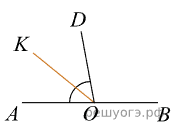
\includegraphics[align=t, width=\textwidth]{\picpath/../../bank/graphs/graph_gleb/Functions/log/1}
		\end{minipage}
		\item Найдите:
		\begin{tasks}
			\task \( 5\sin\alpha \), если \( \cos\alpha=\dfrac{2\sqrt{6}}{5} \) и \( \alpha\in\left( \dfrac{3\pi}{2}; 2\pi \right) \);
			\task \( 3\cos\alpha \), если \( \sin\alpha=-\dfrac{2\sqrt{2}}{3} \) и \( \alpha\in\left( \dfrac{3\pi}{2}; 2\pi \right) \);
			\task \( 24\cos\alpha \), если \( \sin\alpha=-0,2 \);
			\task \( \sin\left( \dfrac{7\pi}{2}-\alpha \right) \), если \( \sin\alpha=0,8 \) и \( \alpha\in\left( \dfrac{\pi}{2}; \pi \right) \).
		\end{tasks}
		\item Первый насос наполняет бак за \(20\) минут, второй --- за \(30\) минут, а третий --- за \(1\) час. За сколько минут наполнят бак три насоса, работая одновременно?
		%\item Игорь и Паша красят забор за \(9\) часов. Паша и Володя красят этот же забор за \(12\) часов, а Володя и Игорь --- за \(18\) часов. За сколько часов мальчики покрасят забор, работая втроем?
		\item Первая труба пропускает на \(8\) литров воды в минуту меньше, чем вторая. Сколько литров воды в минуту пропускает первая труба, если резервуар объемом \(660\) литров она заполняет на \(11\) минут дольше, чем вторая труба заполняет резервуар объемом \(570\) литров?
	\end{listofex}
\end{homework}
%END_FOLD